\documentclass[11pt,a4paper]{article}
\usepackage[margin=25mm]{geometry}
\usepackage{amsmath,amssymb,graphicx,booktabs,tabularx,array}
\usepackage{microtype}
\usepackage{indentfirst}
\usepackage{flafter}
\usepackage{placeins}
\usepackage[numbers,sort&compress]{natbib}
\usepackage[table]{xcolor}
\usepackage{caption}
\usepackage{hyperref}
\definecolor{ink}{HTML}{183344}
\definecolor{teal}{HTML}{217C80}
\hypersetup{colorlinks=true,linkcolor=ink,citecolor=teal,urlcolor=teal,pdftitle={Can Astra Guide a VLA to Solve RoboMME? A Self-Evolving Harness for Memory-Dependent Manipulation}}
\graphicspath{{figures/}}
\newcommand{\citepending}[1]{\citep{#1}}
\newcommand{\pifive}{\ensuremath{\pi_{0.5}}}
% Compact case panels: keep labels readable while reducing image area.
\newenvironment{casefigure}{%
  \par\addvspace{\intextsep}\noindent\begin{minipage}{\linewidth}
  \centering\captionsetup{type=figure,font=small}%
}{\end{minipage}\par\addvspace{\intextsep}}
\newcommand{\caseframe}[3]{%
  \begin{minipage}[t]{0.31\linewidth}\centering
  \includegraphics[width=0.72\linewidth]{supplementary/20261023-stopcube/figures/#1-front.png}\par
  \vspace{2pt}{\scriptsize #2\par #3\par}
  \end{minipage}}
\setlength{\emergencystretch}{2em}
\title{Can Astra Guide a VLA to Solve RoboMME?\\[3pt]
\large A Self-Evolving Harness for Memory-Dependent Manipulation}
\author{}
\date{Technical report}
\begin{document}
\maketitle
\begin{abstract}
Robot manipulation often requires information from past observations to guide current actions. We present a self-evolving harness that combines GPT-6 Astra with the official RoboMME GroundSG vision-language-action model (VLA) for memory-dependent manipulation. Astra interprets task history and selects subgoals, while the VLA handles their execution. To reduce repeated supervision, Astra chooses how many control steps the VLA may execute before review and can select robot-state monitors that prompt earlier inspection. It also intervenes directly when execution requires correction. Starting from subtask-duration priors, the harness accumulates and revises experience across episodes. This experience informs when Astra can rely on the VLA and when closer supervision is needed, while VLA weights remain fixed. Across 800 test episodes covering all 16 RoboMME tasks, the system achieves 97.1\% success, with 54.9\% of control steps executed without additional Astra review. These results show that high task success can coexist with less frequent supervision, supporting experience-guided coordination as a practical way to combine VLM reasoning with learned robot control.
\end{abstract}
\begin{figure}[!t]
\centering
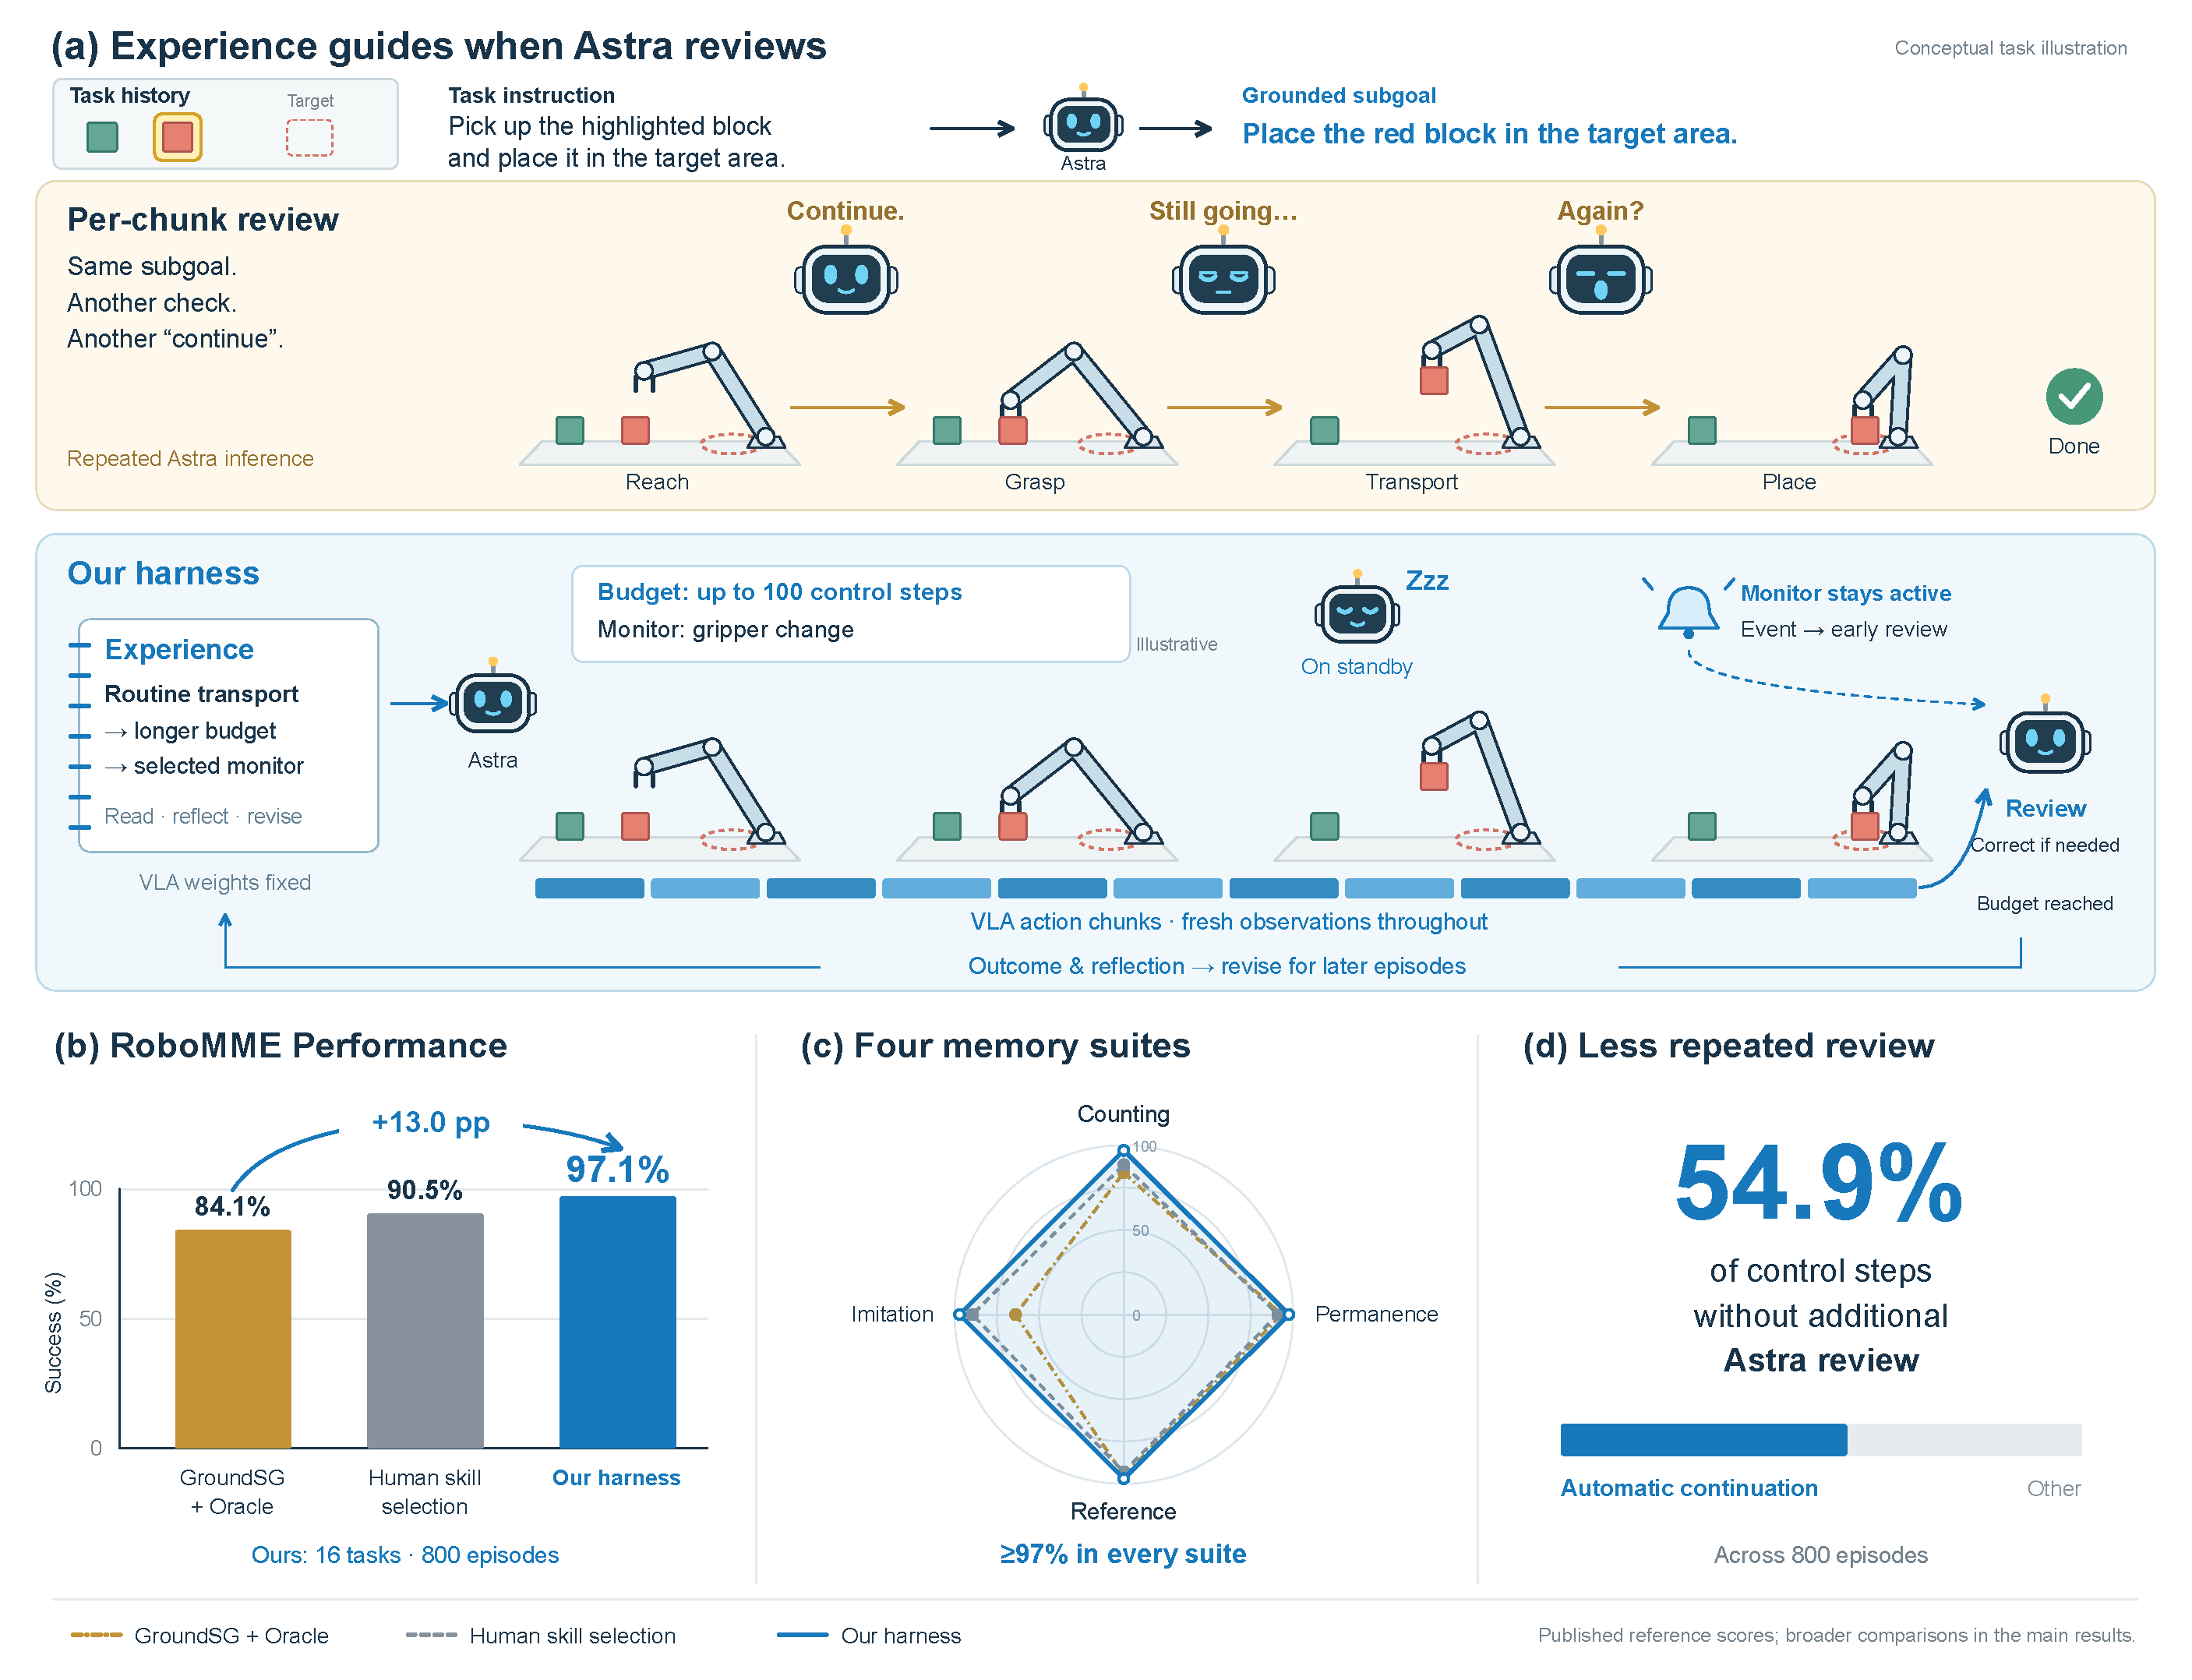
\includegraphics[width=\linewidth]{teaser.pdf}
\captionsetup{font=small,justification=raggedright,singlelinecheck=false}
\caption{Experience-guided supervision of a VLA. (a) Astra interprets task history, delegates execution with a finite budget and selected monitors, and revises experience for later episodes. The scene and budget are illustrative; monitor events can prompt earlier review. (b,c) Success compared with the published RoboMME human skill-selection and GroundSG+Oracle references; Table~\ref{tab:performance} gives broader comparisons. (d) Automatic continuation accounts for 54.9\% of executed control steps across 800 episodes.}
\label{fig:teaser}
\end{figure}
\section{Introduction}
\label{sec:introduction}
In robotic manipulation, deciding what to do next often requires information from past observations. A robot may need to remember which container hides a target, count earlier events, or reproduce a demonstrated action sequence. RoboMME evaluates these capabilities through 16 tasks grouped into counting, permanence, reference, and imitation \citepending{robomme}. Solving them requires both interpreting the relevant history and executing actions consistent with it.

Recent RoboMME studies use GPT-6 Astra (hereafter Astra), a vision-language reasoning model, in two distinct roles. Direct control asks Astra to generate robot motion targets from visual history, placing action generation as well as task reasoning in the model and incurring repeated inference during execution \citepending{astra-direct}. A three-tier system instead uses Astra to plan subgoals for a trained vision-language-action model (VLA), with a separate learned monitor tracking completion \citepending{astra-three-tier}. This division reduces Astra's involvement in routine motion, but concentrates its role on planning. We seek to retain the efficiency of learned control while also using Astra to supervise progress and intervene when execution goes wrong.

Reviewing every short action sequence, or action chunk, incurs repeated inference cost even when the VLA is still executing the same subgoal. Longer intervals between reviews can delay correction of a failed grasp or an incorrect motion. Appropriate supervision therefore depends on the current task stage, visual evidence, and the controller's behavior in similar situations. Experience from earlier episodes can help guide these decisions, but must be updated when new outcomes reveal its limitations.

We present a self-evolving harness in which Astra learns from execution experience how to supervise the official RoboMME GroundSG VLA (Figure~\ref{fig:teaser}). Given task history and current observations, Astra selects a subgoal and a finite execution budget. When permitting a longer interval, it can activate auxiliary monitors, such as gripper-state or directional-motion checks, to trigger review before the budget expires. The VLA continues to react to the latest observations throughout this interval. At review, Astra decides whether to continue execution, revise the subgoal, or intervene directly. Post-episode reflection revises advice about these choices, progressively informing supervision without changing VLA weights.

We evaluate the harness on all 16 RoboMME tasks with 50 episodes per task. It achieves 97.1\% success across 800 episodes, reaches at least 90\% on every task, and executes 54.9\% of control steps without additional Astra review. Execution and experience traces show how prior outcomes lead to revised review intervals and more specific task interpretations. Together, these results and traces illustrate how experience can guide Astra's supervision while the VLA carries out substantial portions of execution without additional review.

\section{Related work}
\label{sec:related}
\paragraph{Foundation models for robot control.}
Language and vision-language models connect high-level task reasoning to robot execution through affordance-based skill selection, robot API programs, and spatial objectives for motion planning \citepending{saycan,code-as-policies,voxposer}. VLAs learn action prediction from robot demonstrations and pretrained representations \citepending{rt2,openvla,pi05}, while RoboICL and GPT-Policy explore general-purpose VLM control from demonstrations and feedback without deployment-time weight updates \citepending{roboicl,gpt-policy}. The direct Astra policy generates Cartesian waypoints using sampled episode history on RoboMME \citepending{astra-direct}. In our system, a trained VLA handles routine execution, while Astra can directly intervene when needed.

\paragraph{Hierarchical execution and feedback.}
Inner Monologue incorporates environmental feedback into language-based planning \citepending{inner-monologue}. PonderPounce uses a multimodal model to maintain episode context and guide a fast VLA, while $\tau_0$-VLA combines execution memory with world-model-guided subtask selection \citepending{ponderpounce,tau0-vla}. The three-tier Astra system uses a fine-tuned Qwen3-VL-4B monitor to detect subtask completion and trigger the next Astra planning call, while a fine-tuned \pifive\ executes the subtasks \citepending{astra-three-tier}. In contrast, our harness allows Astra to schedule execution reviews and configure auxiliary monitors that can trigger earlier inspection. Beyond subtask completion, Astra can assess execution errors and intervene directly when recovery is needed.

\paragraph{Task memory and experience reuse.}
RoboMME evaluates manipulation that depends on past observations \citepending{robomme}. Relevant memory mechanisms include SAM2Act+'s visual memory bank, MEM's short-horizon video and long-horizon text, SimpleMemVLA's sampled video context, and MemER's retrieval of task-relevant historical keyframes \citepending{sam2act,mem,simplememvla,memer}. Our harness uses archived images and episode notes to maintain task context within an episode, while separately accumulating experience to guide decisions in future episodes.

Beyond within-episode memory, Reflexion uses textual feedback to improve subsequent attempts, Voyager accumulates reusable skills through interaction, and ME-Brain-1.0 consolidates embodied experience for future decisions \citepending{reflexion,voyager,mebrain}. Our persistent store contains conditional execution advice that Astra can revise after an episode. This experience guides subgoal planning, review timing, and recovery decisions, with recommendations tied to their supporting evidence and applicable conditions.

\section{Harness}
\label{sec:harness}

\subsection{System and task context}

The harness combines Astra's task reasoning and supervision with VLA execution and direct intervention (Figure~\ref{fig:architecture}). The system uses the official RoboMME GroundSG checkpoint for low-level control, while Astra selects subgoals, supervises execution, and intervenes directly when needed.

Before each Astra review, the VLA predicts an action sequence from the current observations and subgoal. The harness uses forward kinematics to estimate the corresponding end-effector motion, making the predicted actions easier for Astra to interpret. Astra then receives the task instruction, current front and wrist RGB images, robot state, and a summary of the VLA's predicted motion. It can also query archived observations and consult episode notes and relevant experience before making its next decision.

\begin{figure}[!htbp]
\centering
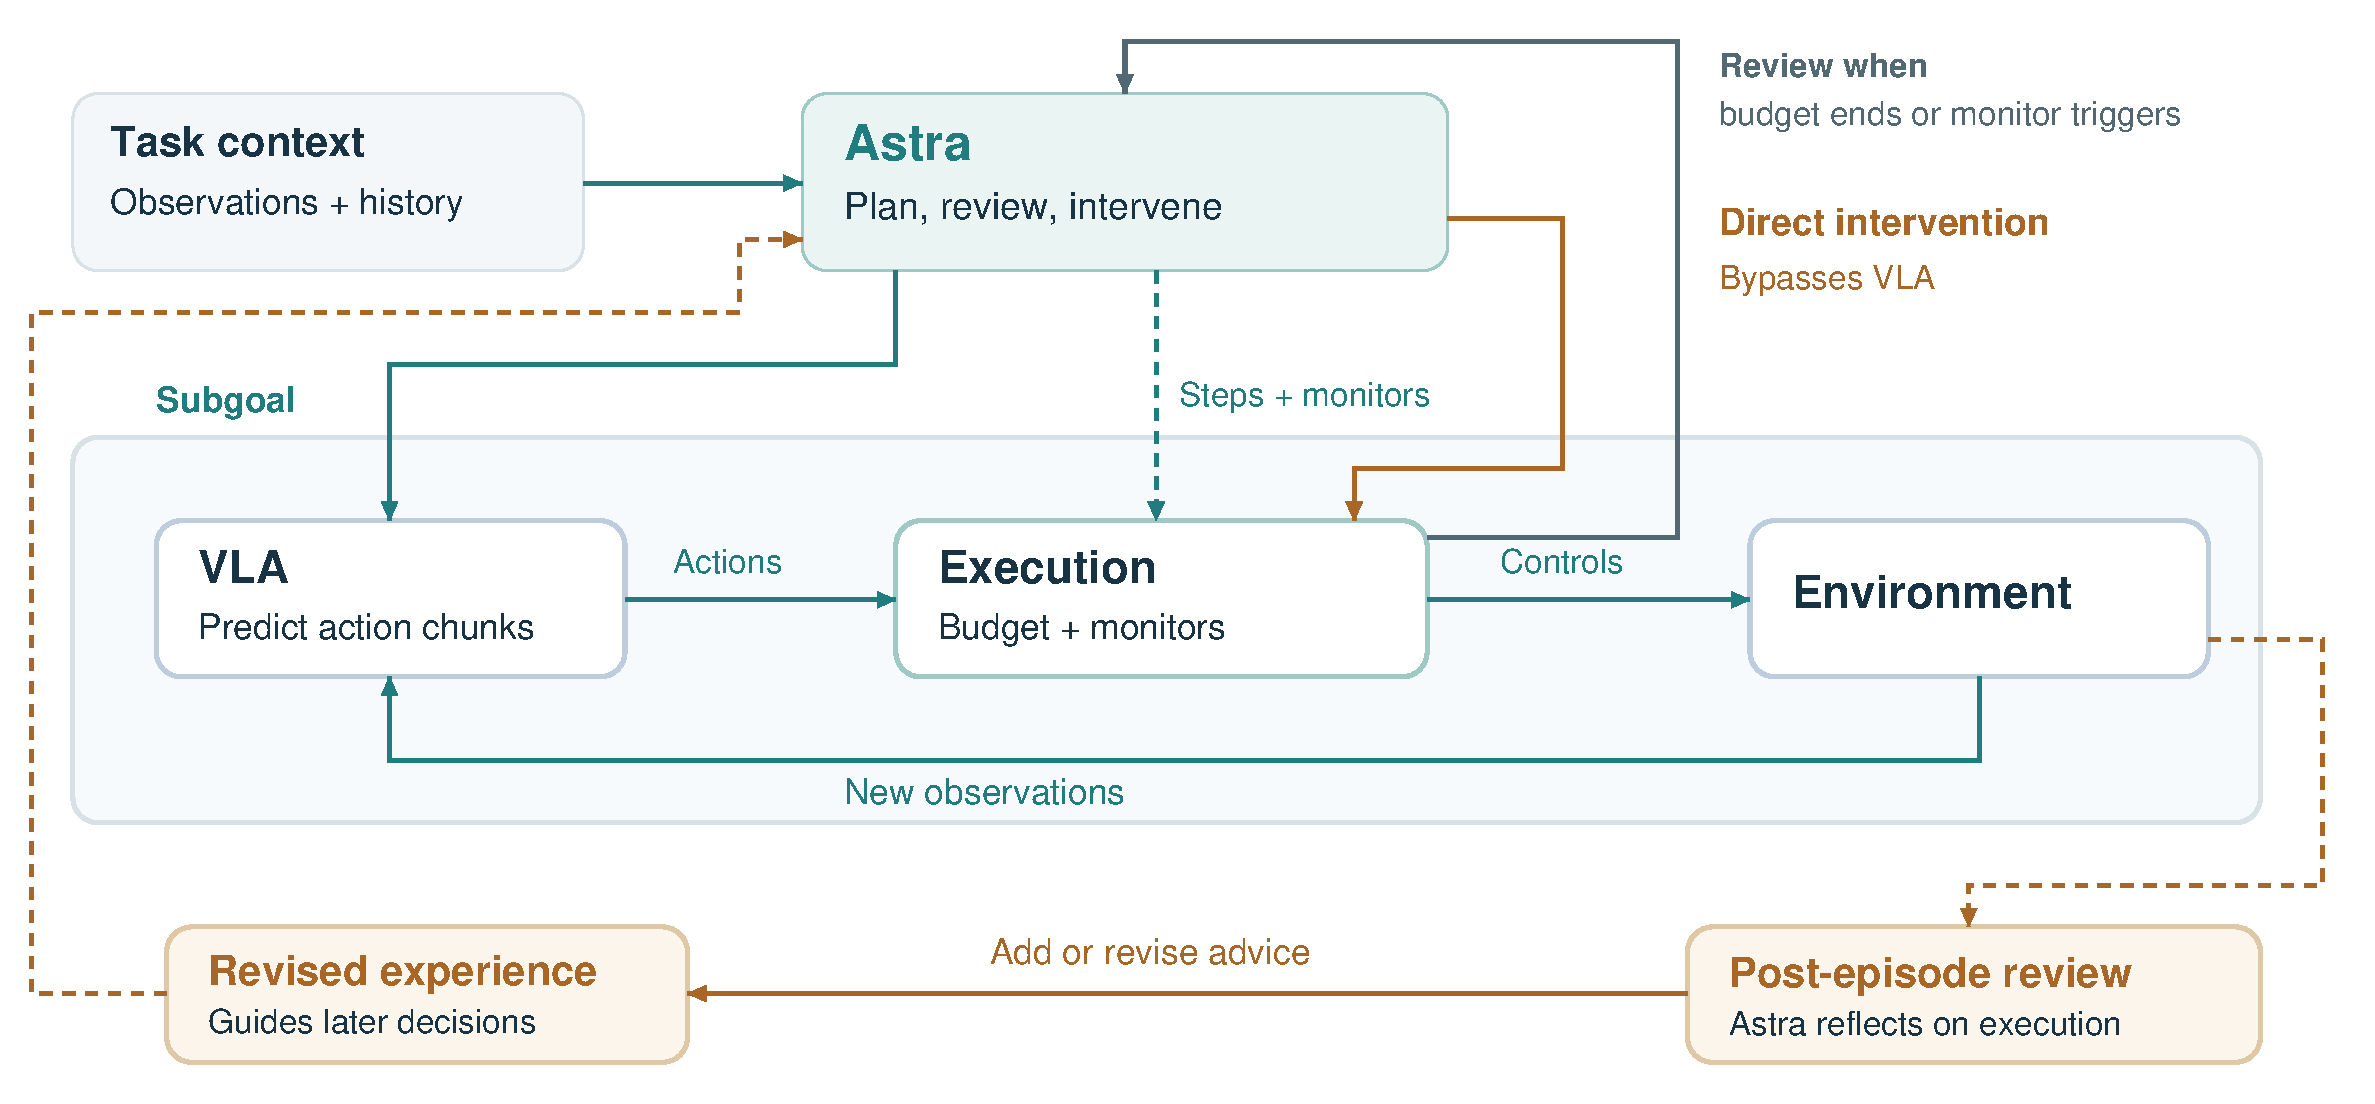
\includegraphics[width=\linewidth]{architecture.pdf}
\caption{Astra assigns execution budgets and selects monitors while the VLA responds to updated observations. Direct interventions bypass the VLA, and post-episode review revises experience for subsequent episodes.}
\label{fig:architecture}
\end{figure}

Astra can authorize a single action chunk, delegate multiple chunks before the next review, or directly issue end-effector targets in world coordinates and gripper commands. After a subgoal change or direct intervention, the VLA predicts a new action sequence using the latest observation and current subgoal before execution resumes.

History queries retrieve information no longer visible in the current observations, including reset demonstrations and intermediate frames. Astra initially samples frames from a requested interval, including its endpoints, and can narrow the interval or inspect individual frames when more detail is needed. Episode notes preserve task-relevant interpretations, unresolved hypotheses, and references to supporting frames. Global and task-specific experience remains available throughout the episode. All decisions rely on task instructions, RGB observations, and robot state available under standard RoboMME evaluation. The harness does not access privileged information such as ground-truth object states or oracle subgoals. Episode success is determined by official environment feedback.

\subsection{Grounded subgoals}

A grounded subgoal combines a RoboMME task template, semantic attributes, and target image points \citepending{robomme}. Astra identifies the relevant attributes from task history and the current scene. The harness then converts normalized image points into front-image pixel coordinates for the grounded instruction. For example, an InsertPeg grasp specifies which end of the peg to grasp and its image location:

\begin{quote}
\small\ttfamily\raggedright
pick up the peg by grasping the near end at <128, 64>
\end{quote}

The coordinates are illustrative. The insertion subgoal also specifies the left or right side of the box. The VLA receives the grounded instruction alongside the task instruction, current images, and robot state, following the representation used in its RoboMME training annotations. Applicable experience can guide target selection or recovery, while Astra determines whether the recorded conditions apply to the current scene. Experience can thus influence subgoal selection without changing the task requirements or the VLA's instruction vocabulary. Appendix~\ref{app:interfaces} provides conversion and validation details.

\subsection{Execution delegation and recovery}

To avoid unnecessary reviews during routine execution, Astra assigns a finite execution budget based on current observations, task history, and relevant experience. Initial budget recommendations are derived from subtask durations in the VLA training demonstrations, using the lower quartile of each subtask's duration distribution as a starting point. As experience accumulates, these recommendations are refined for specific task stages and execution difficulties.

For longer execution intervals, Astra can activate auxiliary monitors to detect events that may require attention. These include gripper-state changes, directional displacement beyond a specified threshold, and a lack of end-effector movement. When assigning a budget, Astra selects the relevant monitors, whose triggers prompt visual review before the budget expires. This allows longer periods of routine VLA execution without losing the ability to inspect potentially problematic events. Monitor thresholds and implementation details are provided in Appendix~\ref{app:configuration}.

The budget counts actual executed control steps rather than predicted actions. At chunk $j$, let $b_j$ denote the remaining budget and $h_j$ the number of predicted actions available for execution. We use the official GroundSG evaluation setting of 16 executed steps per action chunk as the maximum chunk length. The number of actions released is
\begin{equation}
 \ell_j=\min(16,h_j,b_j),\qquad b_{j+1}=b_j-u_j,
 \label{eq:budget}
\end{equation}
where $u_j\leq\ell_j$ is the number of actions actually executed. Execution may stop before all released actions are completed. As long as the budget remains and no monitor has triggered a review, the VLA predicts the next action chunk from updated observations. The VLA therefore continues to respond to changes in the scene without requiring Astra to review every chunk.

At each review during execution, Astra compares the latest observations with the intended subgoal and relevant history. It can extend execution, select a new subgoal, authorize one chunk at a time for closer supervision, or intervene directly. An incorrect target, for example, may require another history query and a revised subgoal, while a stalled contact motion may call for a local end-effector correction. After intervention, the VLA resumes from the resulting observation under Astra's next decision. Budgeted execution and event-triggered reviews allow the VLA to handle routine motion while Astra focuses on decisions and recovery.

\subsection{Cross-episode experience evolution}

The experience store records what Astra learns about task interpretation and VLA execution across episodes. Each entry contains an observation or recommendation, its applicable conditions, and references to supporting frames. Experience can guide target identification, execution budgets, monitor selection, and recovery. Existing entries can be revised when new evidence changes their recommendations or applicable conditions, with earlier versions preserved. New findings become available to subsequent episodes.

After each episode, Astra reviews the execution in the same agent session. The review draws on retained interactions and tool responses, episode notes, active experience, and official outcome and termination feedback. Astra can also inspect archived front and wrist images, starting with sparse samples and examining individual intervals in greater detail when needed. Execution records preserve selected budgets, executed steps, and review triggers. These records help Astra identify problematic stages and reconsider its earlier supervision and recovery decisions.

Based on this review, Astra adds new entries for findings not yet covered by the store and revises existing ones when new evidence changes their recommendations or applicable conditions. For example, hovering before a scheduled review may motivate a shorter budget for that stage or the use of a stationary-motion monitor. Experience from a temporal query may also be refined to distinguish tasks that refer to events before or after a particular observation. These updates turn individual outcomes into more specific guidance for future decisions.

Experience updates undergo structural and scope checks before being stored. During later episodes, Astra can refer to relevant entries when selecting subgoals, setting execution budgets, or choosing recovery actions. The resulting decisions can be traced back to the experience that informed them (Section~\ref{sec:results}). The harness thus adapts through accumulated and revised experience while keeping the VLA weights fixed.

% \section{Harness}
% \label{sec:harness}
% \subsection{System and task context}
% The harness connects Astra's task decisions to VLA execution and direct intervention (Figure~\ref{fig:architecture}). At each decision point, Astra receives the task instruction, current front and wrist RGB images, robot state, and a summary of the next action sequence predicted by the VLA. It can query archived observations and consult episode notes. Relevant global and task experience remains available throughout the episode. Forward kinematics is used to estimate the end-effector motion implied by the VLA's predicted joint actions. Episode success is determined by official environment feedback.

% \begin{figure}[!htbp]
% \centering
% 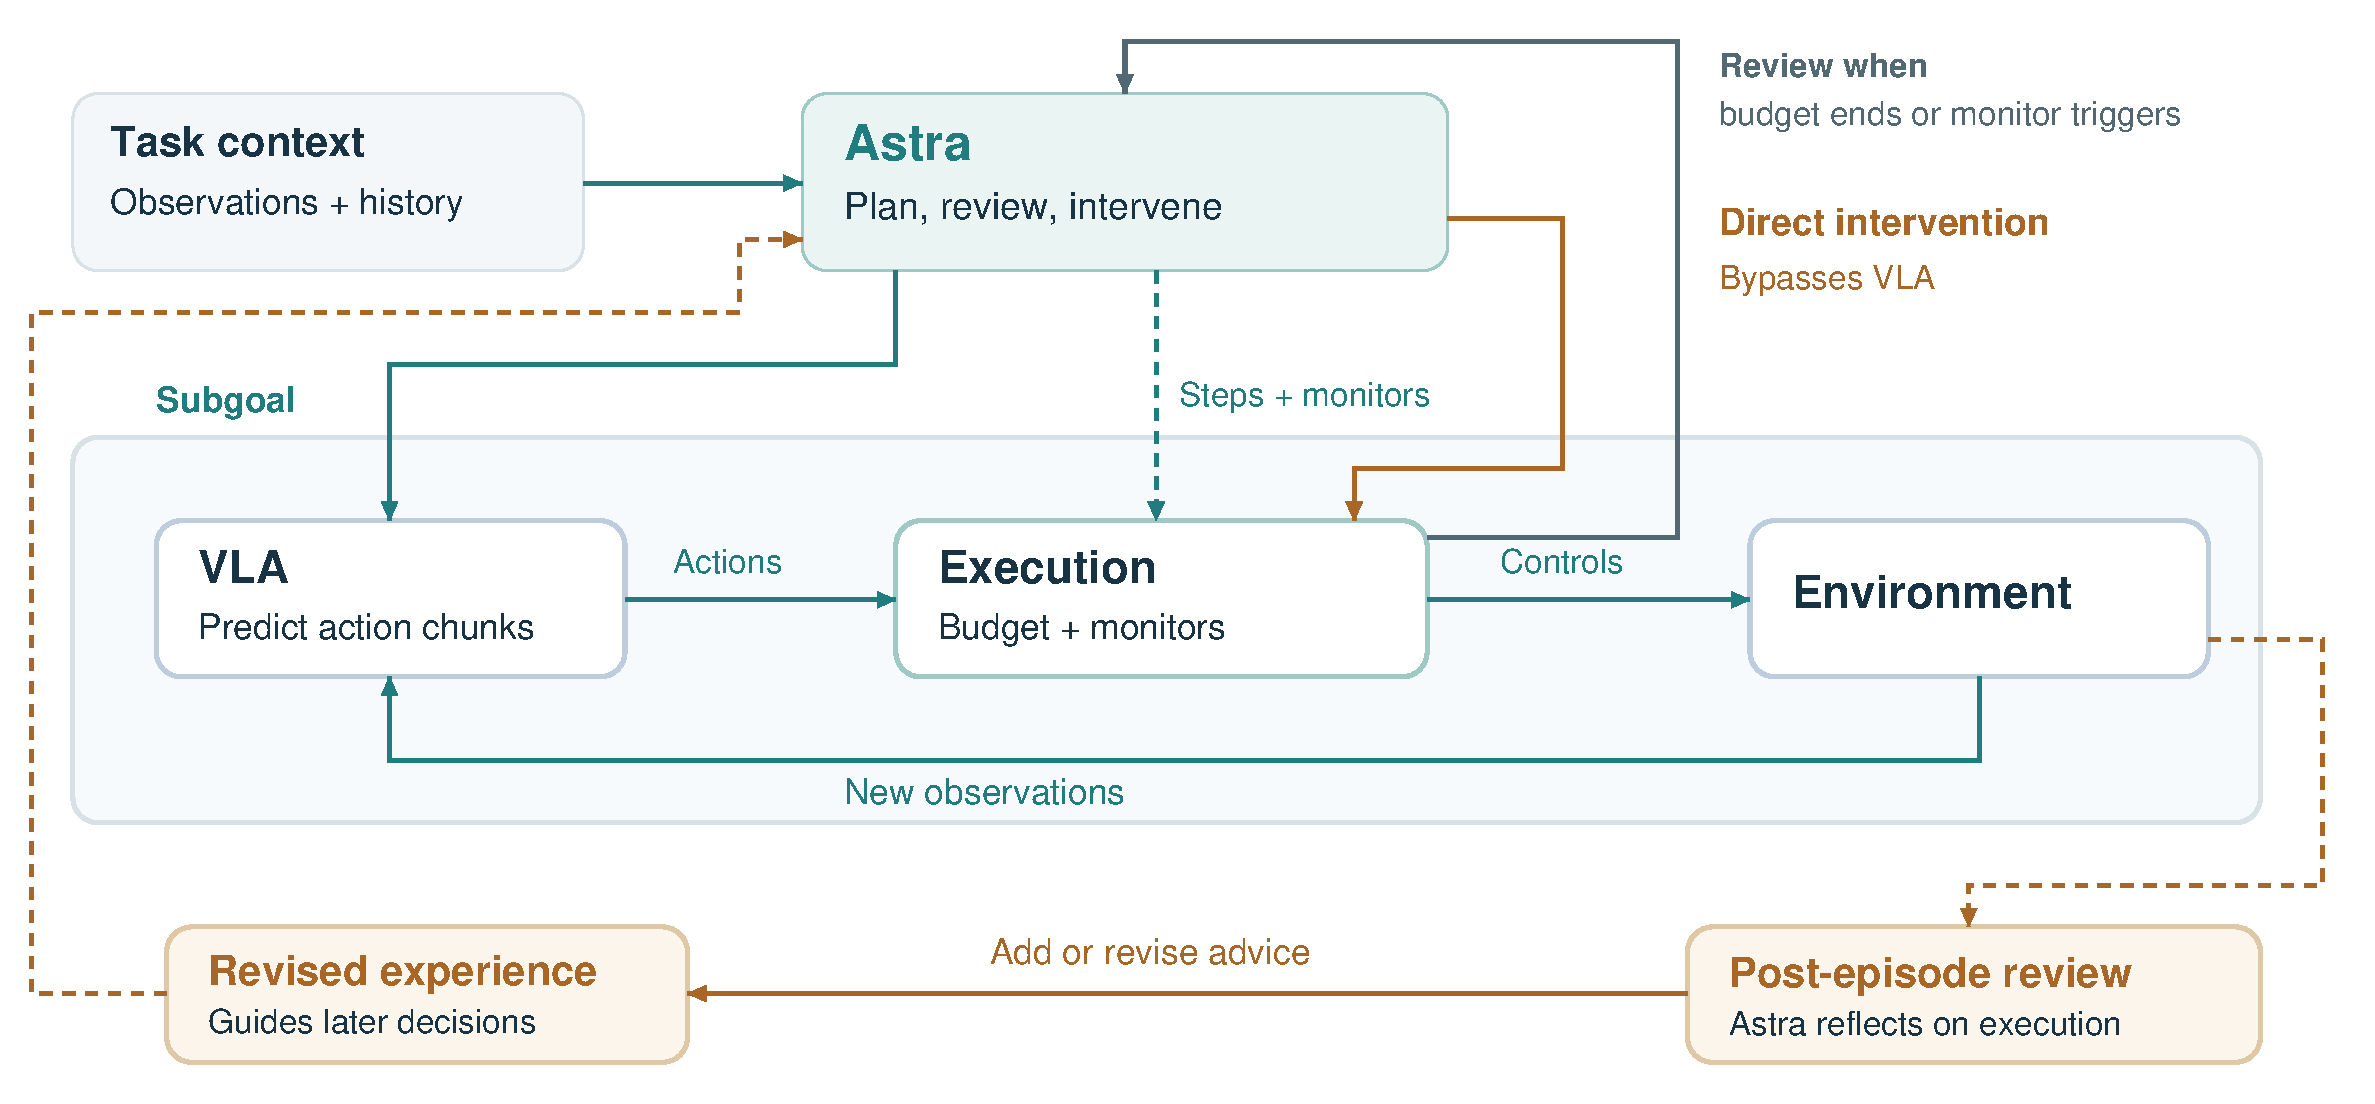
\includegraphics[width=\linewidth]{architecture.pdf}
% \caption{Astra sets execution budgets and selects monitors while the VLA reacts to new observations. Direct interventions bypass the VLA; post-episode review revises advice for later decisions.}
% \label{fig:architecture}
% \end{figure}

% The VLA uses the official RoboMME GroundSG checkpoint and maps its current observation and grounded subgoal to a joint-action sequence. Astra can permit one action chunk, let the VLA execute several chunks before review, or directly specify end-effector targets in world coordinates and gripper commands. Direct intervention bypasses the VLA but acts on the same robot and episode. After a subgoal change or direct intervention, the VLA predicts a new action sequence from the latest observation and current subgoal before execution resumes.

% History queries recover evidence absent from the current views, including reset demonstrations and intermediate observations. Astra first samples a requested interval, including its endpoints, then narrows the interval or inspects original frames when necessary. Episode notes retain task-relevant interpretations and unresolved hypotheses with frame references, allowing Astra to revisit their supporting observations when needed. The agent uses task instructions, front and wrist images, and robot state available under standard RoboMME evaluation. It receives no privileged environment information such as ground-truth object states or oracle subgoals.

% \subsection{Grounded subgoals}
% A grounded subgoal combines a RoboMME task template, semantic attributes, and target image points \citepending{robomme}. Astra resolves the attributes from history and the current scene; the harness converts normalized points to front-image pixel coordinates and inserts them into the instruction. For example, an InsertPeg grasp specifies the near or far end of the peg and its image location:
% \begin{quote}
% \small\ttfamily\raggedright pick up the peg by grasping the near end at <128, 64>
% \end{quote}
% The coordinates here are illustrative image references. Insertion additionally specifies the left or right side of the box. The VLA receives this grounded instruction with the task instruction, current images, and robot state, matching the representation used in its RoboMME training annotations. Applicable experience can advise target selection or recovery, while Astra judges whether its conditions fit the scene. Experience can therefore influence which subgoal is selected without changing the task requirements or the controller's instruction vocabulary. Appendix~\ref{app:interfaces} gives conversion and validation details.

% \subsection{Execution delegation and recovery}
% To avoid unnecessary reviews during routine execution, Astra assigns a finite execution budget based on current observations, task history, and relevant experience. Initial budget advice comes from the number of control steps used to complete subtasks in training demonstrations; the lower quartile of each subtask's duration distribution provides a starting point. Subsequent experience refines these recommendations for particular stages and observed execution difficulties.

% Longer execution intervals can be paired with auxiliary monitoring tools. Gripper-state changes, directional displacement beyond a specified threshold, or a lack of end-effector movement can indicate a stage transition or potential execution problem. Astra selects the relevant monitors when assigning a budget. A detected condition prompts visual review, allowing Astra to inspect progress before the full interval ends. These tools let Astra retain longer budgets during routine motion while watching for events that may require attention. Thresholds and implementation details appear in Appendix~\ref{app:configuration}.

% The budget counts actual executed control steps. At chunk $j$, let $b_j$ be the remaining budget and $h_j$ the number of predicted actions available for execution. Execution uses
% \begin{equation}
%  \ell_j=\min(16,h_j,b_j),\qquad b_{j+1}=b_j-u_j,
%  \label{eq:budget}
% \end{equation}
% where $\ell_j$ is the number of actions released for execution and $u_j\leq\ell_j$ is the number actually executed, which may be smaller if execution stops early. After executing these steps, the VLA predicts the next action chunk from the latest observations. Thus the controller continues to respond to the scene while Astra reviews at the selected interval or when a monitor triggers.

% At a nonterminal review with a valid execution state, Astra compares the new observations with the intended subgoal and relevant history. It can extend execution, choose another subgoal, permit one chunk at a time for close supervision, or intervene directly. For example, an incorrect target may call for another history query and a revised subgoal, whereas a stalled contact motion may call for a local end-effector correction. After intervention, the VLA receives the resulting observation and resumes control under Astra's next decision. Budgeted execution and event-triggered review therefore support both sustained VLA operation and targeted recovery.

% \subsection{Cross-episode experience evolution}
% The experience store captures what Astra learns about task interpretation and VLA execution across episodes. Entries pair an observation or recommendation with its applicable conditions and supporting frames. Advice can concern target identification, review intervals, monitoring choices, or recovery. Revisions replace outdated recommendations while preserving their earlier versions. Each episode uses the available global and task-specific experience, and new findings become available to subsequent episodes.

% After the episode ends, Astra performs the review in the same agent session. Its inputs include retained interactions and tool responses, episode notes, active experience, and the official outcome and termination status. It can query archived front and wrist images, moving from sparse sampling to closer inspection. Execution records include the selected budgets, the number of steps executed, and the conditions that prompted review. Astra uses these records to identify problematic stages, assess its earlier supervision and recovery decisions, and determine whether the findings should update existing experience.

% Astra adds an entry when review identifies a transferable finding, or revises an existing entry when new evidence changes its recommendation or applicable conditions. Findings already covered by the store require no update. For example, hovering observed before a scheduled review can motivate a shorter budget for that phase or the use of a stationary-motion monitor. A recommendation that works for one temporal query can be revised to distinguish before-event and after-event tasks. In this way, experience develops from individual outcomes into conditional guidance for later decisions.

% Updates pass structural and scope checks before entering the experience store. Later decisions can cite the relevant entries when choosing a subgoal, review interval, or recovery action, making it possible to trace how past outcomes informed subsequent actions (Section~\ref{sec:results}). Adaptation takes place through this evolving context while the VLA weights remain fixed.

\section{Experimental setup}
\label{sec:setup}
\paragraph{Benchmark and adaptation.}
We evaluate the official RoboMME test split: 16 tasks across Counting, Permanence, Reference, and Imitation, with 50 episodes per task and 800 in total \citepending{robomme}. Episode seeds and difficulty follow the benchmark specification; official environment feedback determines success. We use GPT-6 Astra as the supervisor and the official RoboMME GroundSG checkpoint, a grounded-subgoal \pifive\ policy, as the VLA. The VLA weights remain fixed. Initial experience consists of duration recommendations derived from subtask completion-step statistics in training demonstrations. In every task, the first five episodes permit experience updates after either outcome; the remaining 45 permit updates only after unsuccessful outcomes. All 50 episodes contribute to the reported success rate. The experience store remains fixed within each episode, and accepted revisions are made available to subsequent episodes. Appendix~\ref{app:configuration} specifies model settings, limits, and cross-task sharing.

\paragraph{Observation access.}
The harness uses the task instruction, front and wrist RGB images, and robot state available to the VLA under standard RoboMME evaluation. Historical observations come from the same observation stream. Planning and control receive no privileged environment ground truth, such as hidden object states or oracle subgoals. Official success and termination feedback is used for outcome assessment and post-episode review.

\paragraph{Comparisons.}
Table~\ref{tab:performance} groups learned policies, direct VLM control, and hierarchical systems, reporting overall success \citepending{robomme,memer,simplememvla,astra-direct,ponderpounce,astra-three-tier}. Human skill selection and GroundSG+Oracle are separate privileged references. PonderPounce-9B uses the reported standard-data leaderboard result, and the other reference scores follow the cited benchmark and system reports; controller training, history access, intervention interfaces, and test-time experience updates differ across systems. We additionally compare delegation with per-chunk review on ten StopCube test seeds. Both conditions are rerun with the same models, history tools, recovery interfaces, and execution limits. Within each pair, both read the same saved version of the experience store, and experience updates are disabled. Runs are serial, with the order of conditions alternating across pairs. This comparison isolates review policy under a fixed experience context for each seed.

\paragraph{Measurements.}
We report task success and the distribution of control steps across four execution modes: subgoal entry, Astra intervention, automatic VLA continuation, and VLA continuation after review. The last mode is the first VLA chunk released after Astra checks progress on the current subgoal; subsequent chunks within the same budget count as automatic continuation. Completion time includes model inference, history queries, action execution, and waiting. Completion-time statistics are reported for successful episodes, since failed runs may terminate early or continue until the execution limit. Appendix~\ref{app:measurements} gives detailed accounting.

\section{Results and analysis}
\label{sec:results}
\subsection{Task performance}
The harness succeeds in 777 of 800 episodes (97.1\%; Table~\ref{tab:performance}), exceeding the published direct-Astra and three-tier Astra scores by 5.0 and 18.0 percentage points, respectively. Success reaches 97.0\% on Counting, 97.5\% on Permanence, and 97.0\% on both Reference and Imitation. Every task achieves at least 90\%, and seven reach 50/50 successes. Gains over direct Astra are particularly large on MoveCube (100\% versus 54\%) and StopCube (96\% versus 54\%). The task results in Figure~\ref{fig:task-comparison} show that the combined system performs well across all four memory categories.

\begin{figure}[!htbp]
\centering
\captionsetup{font=small,justification=raggedright,singlelinecheck=false}
\begin{minipage}[t]{0.37\linewidth}
\vspace{0pt}
\captionof{table}{Overall success on RoboMME (\%).}
\label{tab:performance}
\small
\setlength{\tabcolsep}{4pt}
\renewcommand{\arraystretch}{1.08}
\begin{tabularx}{\linewidth}{@{}Xr@{}}
\toprule
\textbf{Method} & \textbf{Overall} \\
\midrule
\rowcolor{ink!7}\multicolumn{2}{l}{\footnotesize\bfseries Learned policies} \\
\hspace{3pt}\pifive & 17.9 \\
\hspace{3pt}FrameSamp+Modul & 44.5 \\
\hspace{3pt}SAM2Act+ & 21.4 \\
\hspace{3pt}SimpleMemVLA & 88.3 \\
\addlinespace[3pt]
\rowcolor{ink!7}\multicolumn{2}{l}{\footnotesize\bfseries Direct VLM control} \\
\hspace{3pt}Astra & 92.1 \\
\addlinespace[3pt]
\rowcolor{ink!7}\multicolumn{2}{l}{\footnotesize\bfseries Hierarchical systems} \\
\hspace{3pt}MemER & 42.4 \\
\hspace{3pt}GroundSG+QwenVL & 32.7 \\
\hspace{3pt}GroundSG+Gemini & 11.6 \\
\hspace{3pt}PonderPounce-9B & 60.8 \\
\hspace{3pt}Three-tier Astra & 79.1 \\
\rowcolor{blue!7}\hspace{3pt}\textcolor{blue!65!black}{\textbf{Our harness}} & \textbf{97.1} \\
\addlinespace[3pt]
\rowcolor{ink!7}\multicolumn{2}{l}{\footnotesize\bfseries Privileged references} \\
\hspace{3pt}Human & 90.5 \\
\hspace{3pt}GroundSG+Oracle & 84.1 \\
\bottomrule
\end{tabularx}
\end{minipage}\hfill
\begin{minipage}[t]{0.60\linewidth}
\vspace{0pt}
\centering
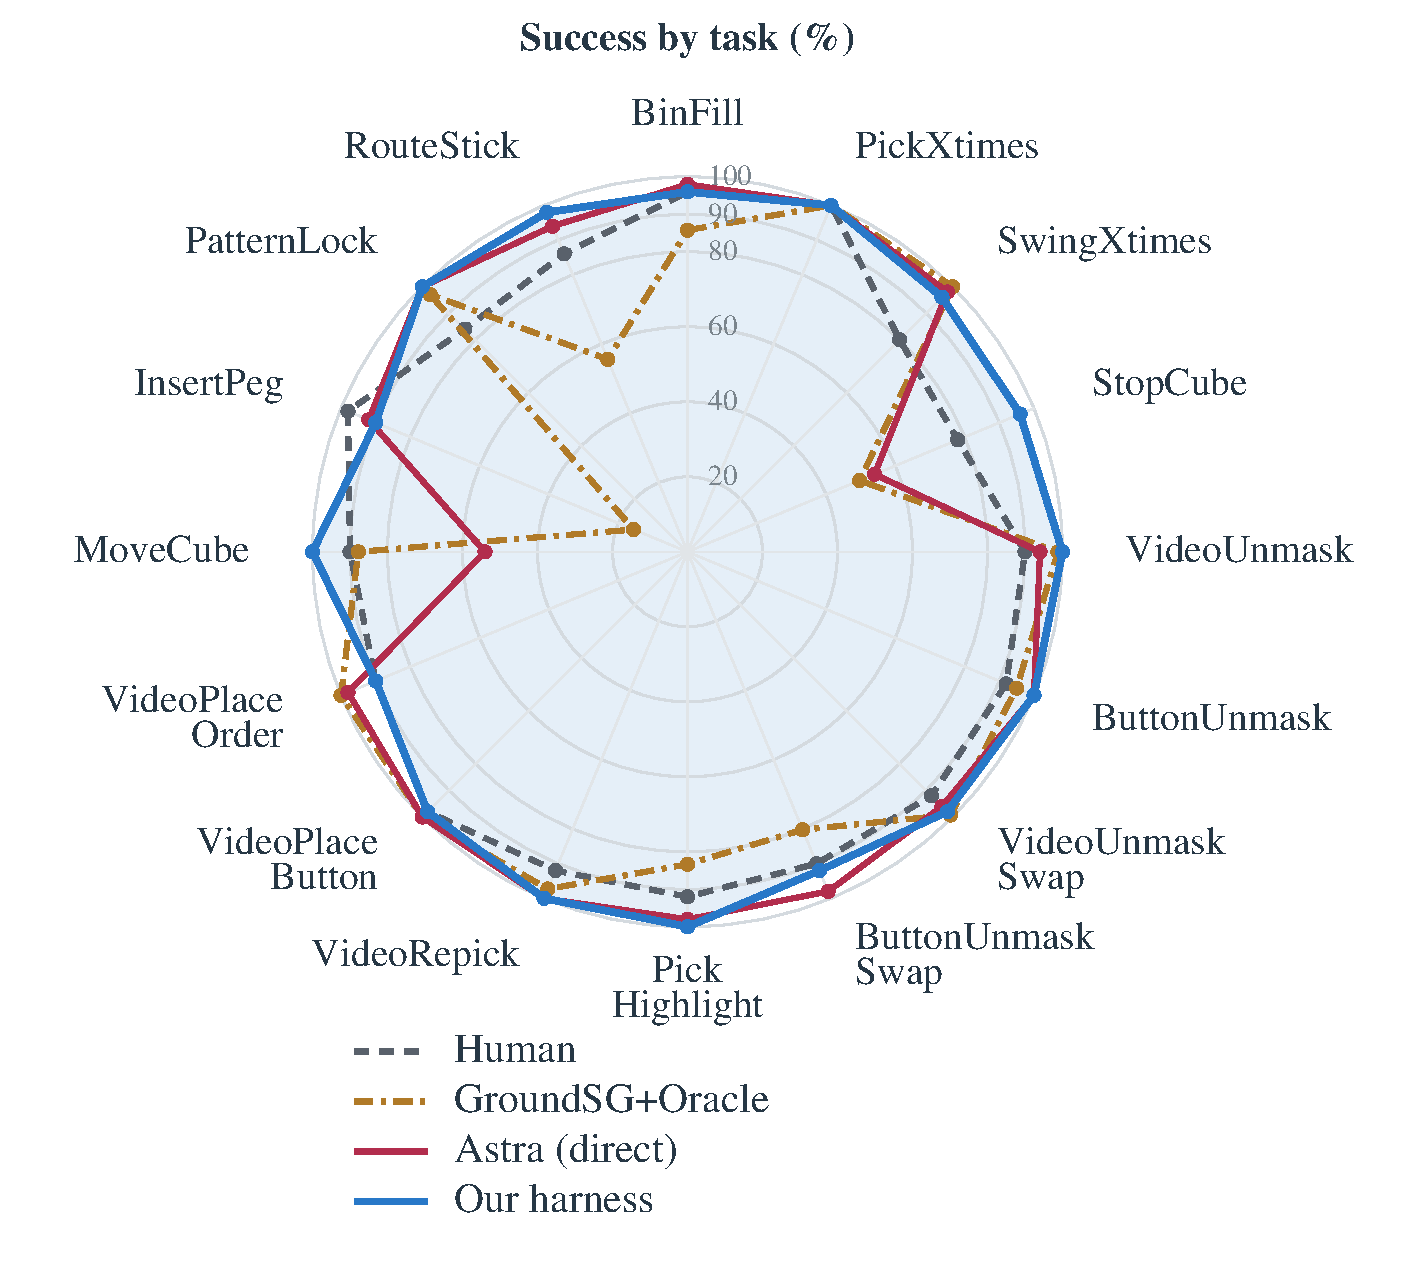
\includegraphics[width=\linewidth]{task_comparison.pdf}
\captionof{figure}{Per-task success of our harness and published references \citepending{robomme,astra-direct}. Human uses an oracle skill interface; GroundSG+Oracle supplies true subgoals to a learned policy; Astra directly specifies waypoints.}
\label{fig:task-comparison}
\end{minipage}
\end{figure}

\FloatBarrier
\subsection{Supervision and execution efficiency}
Automatic VLA continuation accounts for 54.93\% of control steps, allowing more than half of execution to proceed without additional Astra review (Table~\ref{tab:allocation}). Astra intervenes directly in 33.5\% of episodes, but these interventions account for only 4.91\% of control steps. Most motion therefore remains with the learned controller, while Astra contributes local corrections when needed.

\begin{table}[!htbp]
\centering
\caption{Distribution of executed control steps across 800 episodes. Automatic continuation proceeds without an additional Astra review.}
\label{tab:allocation}
\small
\begin{tabularx}{0.85\linewidth}{@{}Xr@{}}
\toprule
Execution mode & Control steps (\%) \\
\midrule
Subgoal entry & 17.23 \\
Astra intervention & 4.91 \\
Automatic VLA continuation & 54.93 \\
VLA continuation after review & 22.93 \\
\bottomrule
\end{tabularx}
\end{table}

Review frequency adapts to the demands of each task. Insertion involves error-prone contact and alignment, so InsertPeg often requires close inspection and corrective action. RouteStick instead contains short directional subtasks; Astra tends to permit one chunk at a time to avoid continuing past a subtask boundary. In VideoPlaceButton, Astra can allow longer execution intervals once the target has been identified. These patterns suggest that review needs vary across task stages, with some stages requiring closer supervision than others.

Appendix~\ref{app:completion-time} reports full-benchmark completion times. We use a matched comparison to examine the effect of review frequency on execution time and model usage.

\paragraph{Matched review-policy comparison.}
Delegation reduces completion time on the nine StopCube seeds that succeed under both review policies (Table~\ref{tab:paired}). Mean execution time falls from 513.2 to 285.6\,s, a reduction of 44.3\%, and delegation is faster in all nine pairs. Across all ten seeds, the two conditions execute similar numbers of control steps, while delegation automatically continues 57.6\% of execution requests and reduces total input tokens by 60.7\%. Per-chunk review succeeds on 10/10 seeds and delegation on 9/10. This comparison shows that delegation can substantially reduce execution time and token usage, although it fails on one seed completed successfully by per-chunk review.

\begin{table}[!htbp]
\centering
\caption{StopCube review-policy comparison on ten matched seeds with experience updates disabled. Timing uses successful episodes; the paired row uses the nine seeds successful in both conditions. Token counts include cached input and cover execution across all ten episodes.}
\label{tab:paired}
\small
\begin{tabularx}{\linewidth}{@{}Xrr@{}}
\toprule
Measurement & Per-chunk review & Delegation \\
\midrule
Successes / episodes & 10/10 & 9/10 \\
Successful episodes: mean time (s) & 512.0 & 285.6 \\
Successful episodes: median / P90 (s) & 548.8 / 727.0 & 240.2 / 392.0 \\
Jointly successful seeds: mean time (s) & 513.2 & 285.6 \\
Automatic / all requests (\%) & 0.0 & 57.6 \\
Mean control steps / episode & 202.1 & 201.0 \\
Total input tokens (millions) & 30.63 & 12.05 \\
Uncached input tokens (millions) & 2.22 & 1.19 \\
\bottomrule
\end{tabularx}
\end{table}

\FloatBarrier
\subsection{Execution and experience analysis}
Across the evaluation, Astra updates the experience store after 37 episodes, producing 43 entries, including seven revisions of earlier advice. Later execution decisions explicitly cite 38 of these entries across 468 episodes. The cases below show how this reused experience changes review intervals and target interpretation, helping Astra adapt its supervision to the VLA's observed behavior.

\paragraph{Revising execution advice.}
In PickXtimes, Astra observes hovering during button pressing and subsequently adds a stationary-motion monitor to the recommended 90-step budget. In the next episode, execution again reaches the 90-step budget without triggering the monitor. The recorded motion never satisfies the 2\,mm stationary threshold over a 32-step window: the smallest position diameter is 26.9\,mm. Astra revises the advice to 60 initial steps, with review intervals of at most 16 steps during contact or recovery. In the following episode, Astra explicitly cites the revision and sets a 60-step budget with the stationary-motion monitor enabled. The VLA executes four chunks of 16, 16, 16, and 12 steps before budget exhaustion; Astra then permits another action chunk, which completes the task after 13 steps. Figure~\ref{fig:trace} illustrates this revision and subsequent execution. The revised advice brings visual review forward while retaining stationary-motion monitoring as another way to trigger review.

\begin{figure}[!t]
\centering
\captionsetup{font=small}
\caseframe{PickXtimes-ep0-f689}{\textbf{Episode 0} / frame 689}{Hovering inspected after execution}\hfill
\caseframe{PickXtimes-ep1-f284}{\textbf{Episode 1} / frame 284}{90-step budget; monitor does not trigger}\hfill
\caseframe{PickXtimes-ep2-f288}{\textbf{Episode 2} / frame 288}{Review after the revised 60-step budget}
\caption{Experience revision across three PickXtimes episodes. Hovering motivates adding a stationary-motion monitor; continued motion prevents it from triggering in episode 1. Astra then shortens the budget from 90 to 60 steps and adopts this advice in episode 2. Figure~\ref{fig:within-episode-cases}(a) follows episode 2 from review to completion.}
\label{fig:trace}
\end{figure}

\paragraph{Revising historical interpretation.}
In VideoPlaceButton, a failed episode leads to advice for tracking visually similar rings through late demonstration swaps, but the resulting recommendation incorrectly assumes a before-press query. In the next episode, the task asks for the first event after the press; Astra recognizes that the earlier rule does not apply and subsequently revises it to condition on the current temporal query. A later episode asks for the last event before the press. Astra explicitly cites the revision in its notes and execution decision, examines the relevant historical frames, and selects the topmost ring. With an 80-step budget, the VLA completes the task after 54 steps. The revision preserves the identity-tracking advice while making target selection conditional on the requested temporal relation (Figure~\ref{fig:history-case}).

\begin{casefigure}
\caseframe{VideoPlaceButton-ep3-f700}{\textbf{Episode 3} / frame 700}{Late swap inspected after failure}\hfill
\caseframe{VideoPlaceButton-ep4-f501}{\textbf{Episode 4} / frame 501}{First-after query exposes the rule's limit}\hfill
\caseframe{VideoPlaceButton-ep10-f1006}{\textbf{Episode 10} / frame 1006}{Revised rule used for a last-before query}
\caption{Experience revision across three VideoPlaceButton episodes. The first rule tracks ring identity but assumes a before-press query. A first-after query prompts a conditional revision, later applied to a last-before query. Figure~\ref{fig:within-episode-cases}(b) shows the late swap within episode 3.}
\label{fig:history-case}
\end{casefigure}

\subsection{Failure analysis}
We manually inspect all 23 failed episodes and group their primary causes into historical interpretation (8), subgoal grounding (1), execution (9), and review or recovery (5).

Specifically, historical interpretation accounts for all five VideoPlaceOrder failures and also affects VideoPlaceButton and InsertPeg. The RouteStick grounding error concerns the task's left--right convention. Execution problems include insufficient endpoint motion in two SwingXtimes episodes and insufficient container lift in one VideoUnmaskSwap episode. Two ButtonUnmaskSwap episodes advance before the button action is complete, and the two StopCube failures involve early or missed button timing. Repeated alignment and contact recovery also leave some InsertPeg episodes unsuccessful. These cases identify where history interpretation, progress review, and local correction still need improvement; representative trajectories appear in Figure~\ref{fig:failures}, with further details in Appendix~\ref{app:failure-analysis}.

\FloatBarrier
\section{Discussion and limitations}
Despite high task success and less frequent Astra review, the harness has several limitations. On-demand history queries avoid including the entire observation history in every Astra reasoning context. Sparse sampling can nevertheless omit a brief event or a late target swap, leading Astra to choose the wrong subgoal. More targeted retrieval of historical observations could reduce these errors without requiring the entire history to be included in the context.

Experience revision allows Astra to correct advice after new outcomes, yet an incorrect recommendation can still influence subsequent decisions before it is revised. The current store also has no explicit bound on the amount of accumulated advice. As the store grows, redundant or conflicting recommendations may increase context usage and make it harder to select appropriate advice. Retrieval and consolidation that retain useful distinctions while removing redundant advice are natural extensions.

Reducing review frequency addresses only part of the execution overhead. Each Astra decision still requires remote model inference, introducing latency whenever execution pauses for supervisory review. Faster supervisory inference and more selective invocation remain important for approaching the responsiveness of a standalone VLA policy.

\section{Conclusion}
We present a self-evolving harness that uses execution experience to guide Astra's supervision of a learned manipulation policy. Across 800 episodes on all 16 RoboMME tasks, the system achieves 97.1\% success, with 54.9\% of control steps executed without additional Astra review. These results illustrate how accumulated execution experience can inform Astra's review, task interpretation, and recovery decisions, while allowing the VLA to handle most low-level control.

\bibliographystyle{plainnat}
\bibliography{references}
\clearpage
\appendix
\section{Experimental settings}
\label{app:configuration}
Table~\ref{tab:config} specifies the model, experience, and execution settings used in evaluation. We use the official GroundSG checkpoint trained on the RoboMME training split, and training demonstrations also provide the initial duration advice. During testing, experience updates follow the schedule in Section~\ref{sec:setup}. Global advice is shared across tasks, while all 37 accepted updates during the formal evaluation are task-specific. Each episode uses a fixed version of the experience store.

\begin{table}[ht]
\caption{Evaluation settings. Control limits apply to actual executed control steps, including interventions.}
\label{tab:config}
\small
\begin{tabularx}{\linewidth}{@{}p{0.32\linewidth}X@{}}
\toprule
Setting & Value \\
\midrule
Astra model and reasoning setting & GPT-6 Astra; high reasoning effort \\
VLA checkpoint and inference & Official RoboMME GroundSG (\pifive), training step 79,999; inference seed 42 with independent random state per connection \\
Environment control frequency & 20 Hz \\
Camera observations & Front and wrist RGB images \\
Sparse history query & Up to eight uniformly sampled frames, including endpoints \\
Delegation budget range & 30 to 200, in increments of 10 control steps \\
Executed actions per VLA prediction & Up to the first 16 predicted actions, limited by the remaining execution budget \\
Episode API limit & 80 calls; 8,192 output tokens per call; 300,000-token context limit \\
Cross-task experience & Shared global advice and separate task experience; fixed version per episode \\
Paired comparison sample & Ten StopCube seeds; 1,000 control steps per run; no experience updates \\
Compute and serving & Paired experiment: one NVIDIA A100 80GB for the VLA, dual Intel Xeon Platinum 8358P CPUs for simulation; Astra via remote API \\
\bottomrule
\end{tabularx}
\end{table}

\paragraph{Robot-state monitors.}
The measured gripper monitor detects a total finger-width change of at least 5\,mm from the start of the execution interval, sustained for two measured samples in the same direction. The direction monitor checks predicted or measured displacement greater than 20\,mm in a selected signed world-frame direction relative to the robot pose at the start of the execution interval. The stationary-motion monitor uses a position diameter of at most 2\,mm and an orientation diameter of at most $2^\circ$ over 32 control steps. An impending gripper-command switch can also trigger review. Astra selects the active monitors for each execution interval. Budget exhaustion prompts review, and episode termination stops execution.

\section{Per-task performance and execution allocation}
\label{app:task-results}
Table~\ref{tab:task-results} reports success and execution allocation for each task. Automatic continuation counts execution after the first chunk of an execution interval. The control fraction includes direct Astra interventions in its denominator. Each task contributes 50 episodes, and pooled allocation fractions weight tasks by their executed chunk or control counts.

\begin{table}[ht]
\centering
\caption{Per-task results. SR: success rate; auto chunks: automatic continuation as a fraction of all VLA chunks; auto control steps: automatic continuation as a fraction of all executed control steps. All entries are percentages.}
\label{tab:task-results}
\small
\begin{tabular}{@{}llrrr@{}}
\toprule
Category & Task & SR (\%) & Auto chunks (\%) & Auto control steps (\%) \\
\midrule
Counting & BinFill & 96.0 & 63.61 & 60.41 \\
 & StopCube & 96.0 & 65.15 & 68.87 \\
 & PickXtimes & 100.0 & 53.95 & 49.13 \\
 & SwingXtimes & 96.0 & 46.87 & 45.20 \\
\midrule
Permanence & ButtonUnmask & 100.0 & 73.84 & 69.51 \\
 & VideoUnmask & 100.0 & 73.88 & 71.42 \\
 & VideoUnmaskSwap & 98.0 & 69.11 & 65.87 \\
 & ButtonUnmaskSwap & 92.0 & 50.26 & 41.35 \\
\midrule
Reference & PickHighlight & 100.0 & 71.43 & 69.17 \\
 & VideoRepick & 100.0 & 67.55 & 63.03 \\
 & VideoPlaceButton & 98.0 & 76.26 & 75.36 \\
 & VideoPlaceOrder & 90.0 & 63.44 & 65.93 \\
\midrule
Imitation & MoveCube & 100.0 & 53.30 & 48.64 \\
 & InsertPeg & 90.0 & 29.06 & 29.01 \\
 & PatternLock & 100.0 & 35.62 & 34.06 \\
 & RouteStick & 98.0 & 25.65 & 22.30 \\
\midrule
\multicolumn{2}{@{}l}{Overall / pooled} & 97.1 & 58.11 & 54.93 \\
\bottomrule
\end{tabular}
\end{table}

\section{Interface and experience details}
\label{app:interfaces}
\paragraph{Observation provenance.}
Image-delivery records distinguish the visual evidence included in each successful Astra request from observations available only through retrospective inspection of the full recording.

\paragraph{Grounding.}
For a front image of height $H$ and width $W$, a normalized point $(y_n,x_n)\in[0,1000]^2$ is converted to
\begin{equation}
 y=\min(\lfloor y_nH/1000\rfloor,H-1),\qquad
 x=\min(\lfloor x_nW/1000\rfloor,W-1).
\end{equation}
The pixel coordinates replace the instruction's ordered point slots. Validation checks finite coordinate values, normalized bounds, the number of supplied points, and compatibility with the task's templates and permitted attributes. Astra can inspect an overlay before setting the subgoal. The default sparse history query selects up to eight uniformly spaced frames, including interval endpoints.

\paragraph{Control steps and duration priors.}
A control step is counted at the shared environment action interface, separately from simulator integration steps. At environment frequency $f_c=20\,\mathrm{Hz}$, $n$ steps correspond nominally to $n/f_c$ seconds of simulated control. Inference and API waiting time contribute separately to elapsed time. Repeated training samples are deduplicated by task, episode, and timestep before consecutive identical subgoal labels are grouped. Segment lengths are estimated from timestep differences. For lengths $D_s$ associated with subgoal $s$, the initial recommendation is
\begin{equation}
 \widehat B_s=\min\!\left(200,10\left\lfloor Q_{0.25}(D_s)/10\right\rfloor\right).
\end{equation}
Recommendations below 30 control steps become advice for close review. Because sampled annotations may miss short segments or include trailing frames in terminal segments, these duration estimates serve as initial guidance rather than exact subtask boundaries.

\paragraph{Experience validation and applicability.}
Submission checks cover required fields, permitted scope and applicability labels, cited frame indices, and the existence of superseded identifiers. Scheduling advice is also checked for compatibility with subgoal templates and valid monitor parameters. Experience entries are marked as either policy-independent or specific to a review policy. When retrieving advice, the harness first selects entries applicable to the current policy and then resolves superseded recommendations. The optional scheduling field \texttt{max\_trust\_steps} records a recommended review interval; the configured execution maximum remains the enforced limit.

\section{Measurement definitions}
\label{app:measurements}
Success rate is the number of officially successful episodes divided by the evaluated count. Equal task sizes make overall success equal to the mean task success rate. Execution-time summaries include only the 777 successful episodes; token totals include all 800 episodes. API attempts and elapsed time include failed requests. Token statistics report coverage of returned usage; cached input is a subset of total input, and missing usage remains unknown. Execution and post-episode revision token totals are reported separately. API latency for revision is not a measurement of the complete revision wall time.

Automatic continuation counts VLA chunks executed after the first chunk of an execution interval. The all-chunk fraction divides these by all executed VLA chunks. The automatic-control fraction divides control steps in continuation chunks by all executed control steps, including direct interventions. Fractions use pooled counts across episodes rather than averages of episode percentages.

\begin{table}[!htbp]
\centering
\caption{Execution allocation across all 800 episodes. Each row counts executed robot-control requests (VLA chunks or direct intervention segments); direct interventions can have different lengths from VLA chunks. Percentages use pooled counts.}
\label{tab:allocation-detail}
\small
\begin{tabularx}{\linewidth}{@{}Xrrrr@{}}
\toprule
Execution mode & Requests & Share (\%) & Control steps & Share (\%) \\
\midrule
Subgoal entry & 2,829 & 15.88 & 44,709 & 17.23 \\
Astra intervention & 587 & 3.29 & 12,752 & 4.91 \\
Automatic VLA continuation & 10,014 & 56.20 & 142,516 & 54.93 \\
VLA continuation after review & 4,390 & 24.64 & 59,495 & 22.93 \\
\midrule
Total & 17,820 & 100.00 & 259,472 & 100.00 \\
\bottomrule
\end{tabularx}
\end{table}

\FloatBarrier
\section{Successful-episode execution time}
\label{app:completion-time}
Execution time runs from environment readiness to the end of robot execution, excluding startup and post-episode review. The pooled row summarizes all 777 successful episodes, rather than averaging task means. P90 uses linear interpolation between ordered observations.
\paragraph{Interpretation of completion times.}
Across 777 successful episodes, mean completion time is 513.7 seconds, the median is 390.5 seconds, and the 90th percentile is 1,102.0 seconds. Task means range from 141.2 seconds on VideoUnmask to 991.8 seconds on ButtonUnmaskSwap. These measurements include model inference, history queries, action execution, and waiting; API load and network conditions also affect them. These full-benchmark timing results are descriptive and are not intended as controlled efficiency comparisons with published systems. The matched StopCube experiment provides a controlled comparison of review policies.

\begin{table}[!htbp]
\centering\small
\caption{Completion times for successful episodes. All times are seconds.}
\begin{tabular}{@{}lrrrr@{}}
\toprule
Task & Successful episodes & Mean & Median & P90 \\
\midrule
BinFill & 48 & 802.1 & 800.1 & 1378.9 \\
StopCube & 48 & 416.6 & 385.1 & 615.0 \\
PickXtimes & 50 & 712.2 & 602.6 & 1315.3 \\
SwingXtimes & 48 & 887.3 & 913.3 & 1340.5 \\
ButtonUnmask & 50 & 359.0 & 267.4 & 726.2 \\
VideoUnmask & 50 & 141.2 & 111.5 & 237.1 \\
VideoUnmaskSwap & 49 & 383.5 & 288.8 & 690.5 \\
ButtonUnmaskSwap & 46 & 991.8 & 916.6 & 1319.7 \\
PickHighlight & 50 & 385.1 & 352.6 & 610.3 \\
VideoRepick & 50 & 782.9 & 645.0 & 1239.5 \\
VideoPlaceButton & 49 & 306.7 & 281.4 & 413.3 \\
VideoPlaceOrder & 45 & 254.1 & 244.3 & 341.0 \\
MoveCube & 50 & 296.2 & 160.8 & 690.7 \\
InsertPeg & 45 & 760.1 & 719.6 & 1150.8 \\
PatternLock & 50 & 249.5 & 224.4 & 461.0 \\
RouteStick & 49 & 544.1 & 494.0 & 880.1 \\
\midrule
Overall / pooled & 777 & 513.7 & 390.5 & 1,102.0 \\
\bottomrule
\end{tabular}
\end{table}

\FloatBarrier
\section{Monitor selection and resource use}
Monitor selection is counted once per execution interval, across 3,541 intervals. Several monitors may be selected together, so selection shares need not sum to 100\%. No optional monitor is selected in 1,840 intervals (51.96\%); budgets and mandatory termination conditions still apply. Trigger frequency counts intervals ending with a detected condition and does not measure error-detection accuracy.
\begin{table}[!htbp]
\centering\small
\caption{Monitor selection and subsequent triggering. The 28 direction triggers all concern proposed motion; none comes from measured directional displacement.}
\begin{tabularx}{\linewidth}{@{}Xrrr@{}}
\toprule
Monitor & Selected & Share (\%) & Triggered / selected (\%) \\
\midrule
Before gripper-command switch & 1,062 & 29.99 & 28.91 \\
Measured gripper-width change & 354 & 10.00 & 70.34 \\
Selected-direction displacement & 244 & 6.89 & 11.48 \\
Stationary motion & 120 & 3.39 & 0.00 \\
\bottomrule
\end{tabularx}
\end{table}

Selection differs by task stage. On StopCube, all 51 button-preparation intervals omit optional monitors, whereas 56 of 85 stationary-waiting intervals select a direction monitor. On SwingXtimes, a pre-command gripper monitor is selected in 186 of 193 target-movement intervals (96.37\%), compared with 22 of 93 grasping intervals (23.66\%). On PickXtimes, the stationary-motion monitor is selected in 49 of 50 button-stop intervals, yet it never triggers across the evaluation.

\begin{table}[!htbp]
\centering\small
\caption{Mean recorded token usage per evaluated episode, over all 800 episodes. Cached input is a subset of input.}
\begin{tabular}{@{}lrr@{}}
\toprule
Tokens & Execution & Post-episode review \\
\midrule
Input & 1,790,701.2 & 318,456.8 \\
Cached input & 1,633,224.3 & 308,963.6 \\
Uncached input & 157,476.9 & 9,493.2 \\
Output & 2,724.9 & 674.2 \\
\bottomrule
\end{tabular}
\end{table}
All 19,061 successful API responses include usage records, while 112 failed attempts have unknown usage, giving 99.4\% coverage. Reported per-episode means use recorded usage divided by all 800 episodes and may underestimate actual token consumption. They should not be interpreted as billing estimates.

\FloatBarrier
\section{Within-episode case sequences}
\label{app:case-sequences}
Figure~\ref{fig:within-episode-cases} expands the cross-episode examples in Figures~\ref{fig:trace} and~\ref{fig:history-case} with two frames from the same episode in each pair.

\begin{casefigure}
\begin{minipage}[t]{0.48\linewidth}
\centering
{\small\bfseries (a) PickXtimes / episode 2\par}
\vspace{4pt}
\begin{minipage}[t]{0.43\linewidth}\centering
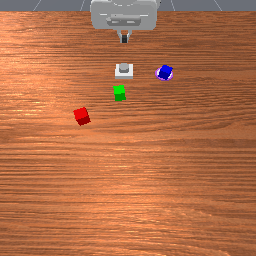
\includegraphics[width=\linewidth]{supplementary/20261023-stopcube/figures/PickXtimes-ep2-f288-front.png}\par
{\scriptsize Frame 288\par Budget exhausted; review\par}
\end{minipage}\hfill
\begin{minipage}[t]{0.43\linewidth}\centering
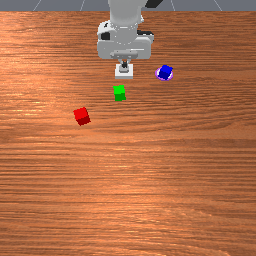
\includegraphics[width=\linewidth]{supplementary/20261023-stopcube/figures/PickXtimes-ep2-f301-front.png}\par
{\scriptsize Frame 301\par Official success\par}
\end{minipage}\par\vspace{4pt}
{\footnotesize $16+16+16+12=60$ steps $\rightarrow$ review\par
Another 13 control steps $\rightarrow$ success\par}
\end{minipage}\hfill
\begin{minipage}[t]{0.48\linewidth}
\centering
{\small\bfseries (b) VideoPlaceButton / episode 3\par}
\vspace{4pt}
\begin{minipage}[t]{0.43\linewidth}\centering
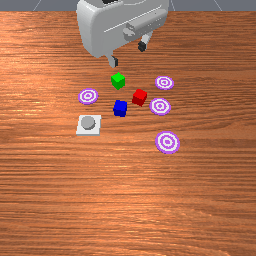
\includegraphics[width=\linewidth]{supplementary/20261023-stopcube/figures/VideoPlaceButton-ep3-f679-front.png}\par
{\scriptsize Frame 679\par Before the late swap\par}
\end{minipage}\hfill
\begin{minipage}[t]{0.43\linewidth}\centering
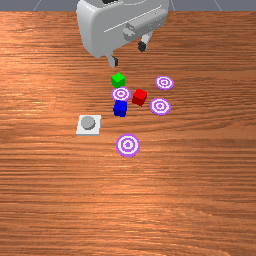
\includegraphics[width=\linewidth]{supplementary/20261023-stopcube/figures/VideoPlaceButton-ep3-f700-front.png}\par
{\scriptsize Frame 700\par After the late swap\par}
\end{minipage}\par\vspace{4pt}
{\footnotesize Late changes in ring positions\par
Both frames inspected after failure\par}
\end{minipage}
\caption{Two within-episode sequences, read left to right within each pair. (a) Astra reviews execution after the revised 60-step budget and permits another chunk; official feedback reports success after 13 further steps. (b) Historical frames show the late ring permutation examined during post-episode review. The pairs document execution and historical evidence, respectively.}
\label{fig:within-episode-cases}
\end{casefigure}

\FloatBarrier
\section{Failure annotation and reference-frame clarification}
\label{app:failure-analysis}
Manual inspection of the 23 unsuccessful episodes assigns one primary label per episode: historical interpretation (8), subgoal grounding (1), execution (9), or review and recovery (5). The execution category includes two SwingXtimes episodes in which the motion does not fully reach the target and one VideoUnmaskSwap episode with insufficient container lift. Each episode is counted once according to its primary failure mode.

In the first RouteStick episode, Astra misinterprets the task's left--right convention, leading to an incorrect directional subgoal. As RoboMME's directional instructions do not explicitly specify the reference frame, we subsequently added a clarification of this convention to the agent's global experience context: task directions refer to the initial wrist view or initial robot orientation, rather than the changing wrist orientation or the front-view screen axes. Image points retain the pixel coordinates of their own camera. This interface clarification is not counted among the 37 autonomous experience updates.

\begin{casefigure}
{\small\bfseries (a) VideoPlaceOrder / episode 11\par}\vspace{3pt}
\caseframe{VideoPlaceOrder-ep11-f491}{Frame 491: remembered location}{Target initially at the lower right}\hfill
\caseframe{VideoPlaceOrder-ep11-f740}{Frame 740: late permutation}{Inspected retrospectively}\hfill
\caseframe{VideoPlaceOrder-ep11-f1012}{Frame 1012: incorrect selection}{Old screen location reused}\par\vspace{8pt}
{\small\bfseries (b) ButtonUnmaskSwap / episode 17\par}\vspace{3pt}
\caseframe{ButtonUnmaskSwap-ep17-f98}{Frame 98: brief button contact}{First button press}\hfill
\caseframe{ButtonUnmaskSwap-ep17-f218}{Frame 218: premature transition}{Container manipulation begins}\hfill
\caseframe{ButtonUnmaskSwap-ep17-f612}{Frame 612: delayed recovery}{Button action revisited}\par\vspace{8pt}
{\small\bfseries (c) InsertPeg / episode 0\par}\vspace{3pt}
\caseframe{InsertPeg-ep0-f441}{Frame 441: incorrect transport}{Direction monitor triggers review}\hfill
\caseframe{InsertPeg-ep0-f633}{Frame 633: alignment attempts}{Contact recovery remains unsuccessful}\hfill
\caseframe{InsertPeg-ep0-f723}{Frame 723: incomplete insertion}{Episode ends without completion}
\caption{Representative failures, read left to right within each episode. (a) VideoPlaceOrder loses target identity through a late ring swap; frame 740 was inspected retrospectively. (b) ButtonUnmaskSwap moves to container manipulation too early and later retries the button. (c) InsertPeg remains incomplete after repeated alignment and contact recovery.}
\label{fig:failures}
\end{casefigure}

\FloatBarrier


\section{Review-policy comparison}
\label{app:paired}
The StopCube comparison uses ten official test seeds, with both policies rerun under the same harness configuration. The two conditions receive identical saved versions of the experience store within each pair. Experience updates are disabled to keep the comparison focused on review policy. Runs alternate which policy executes first.

Delegation is faster on all nine jointly successful seeds, saving a mean of 227.6 seconds. The first per-chunk run includes 35.5 seconds of VLA inference, compared with 2.3 seconds for its delegated counterpart. Excluding this pair leaves eight joint successes with mean times of 491.9 and 280.6 seconds, respectively, a 43.0\% reduction. Across all ten runs, execution uses 2,021 control steps with per-chunk review and 2,010 with delegation. Input-token totals fall from 30.63 to 12.05 million; uncached input falls from 2.22 to 1.19 million, and output from 32,222 to 21,333 tokens.

\end{document}
